\documentclass[10pt,a4paper]{article}
\usepackage[utf8]{inputenc}
\usepackage[magyar]{babel}
\usepackage[T1]{fontenc}
\usepackage{tikz}
\usepackage{pdflscape}
\usepackage[left=2cm,right=2cm,top=2cm,bottom=2cm]{geometry}
\pagenumbering{gobble} 

\begin{document}

\begin{center}
{\Huge \textbf{FELADAT}}
\end{center}

\vspace{0.5cm}

\input{00_leiras.txt}

\newpage

\begin{center}
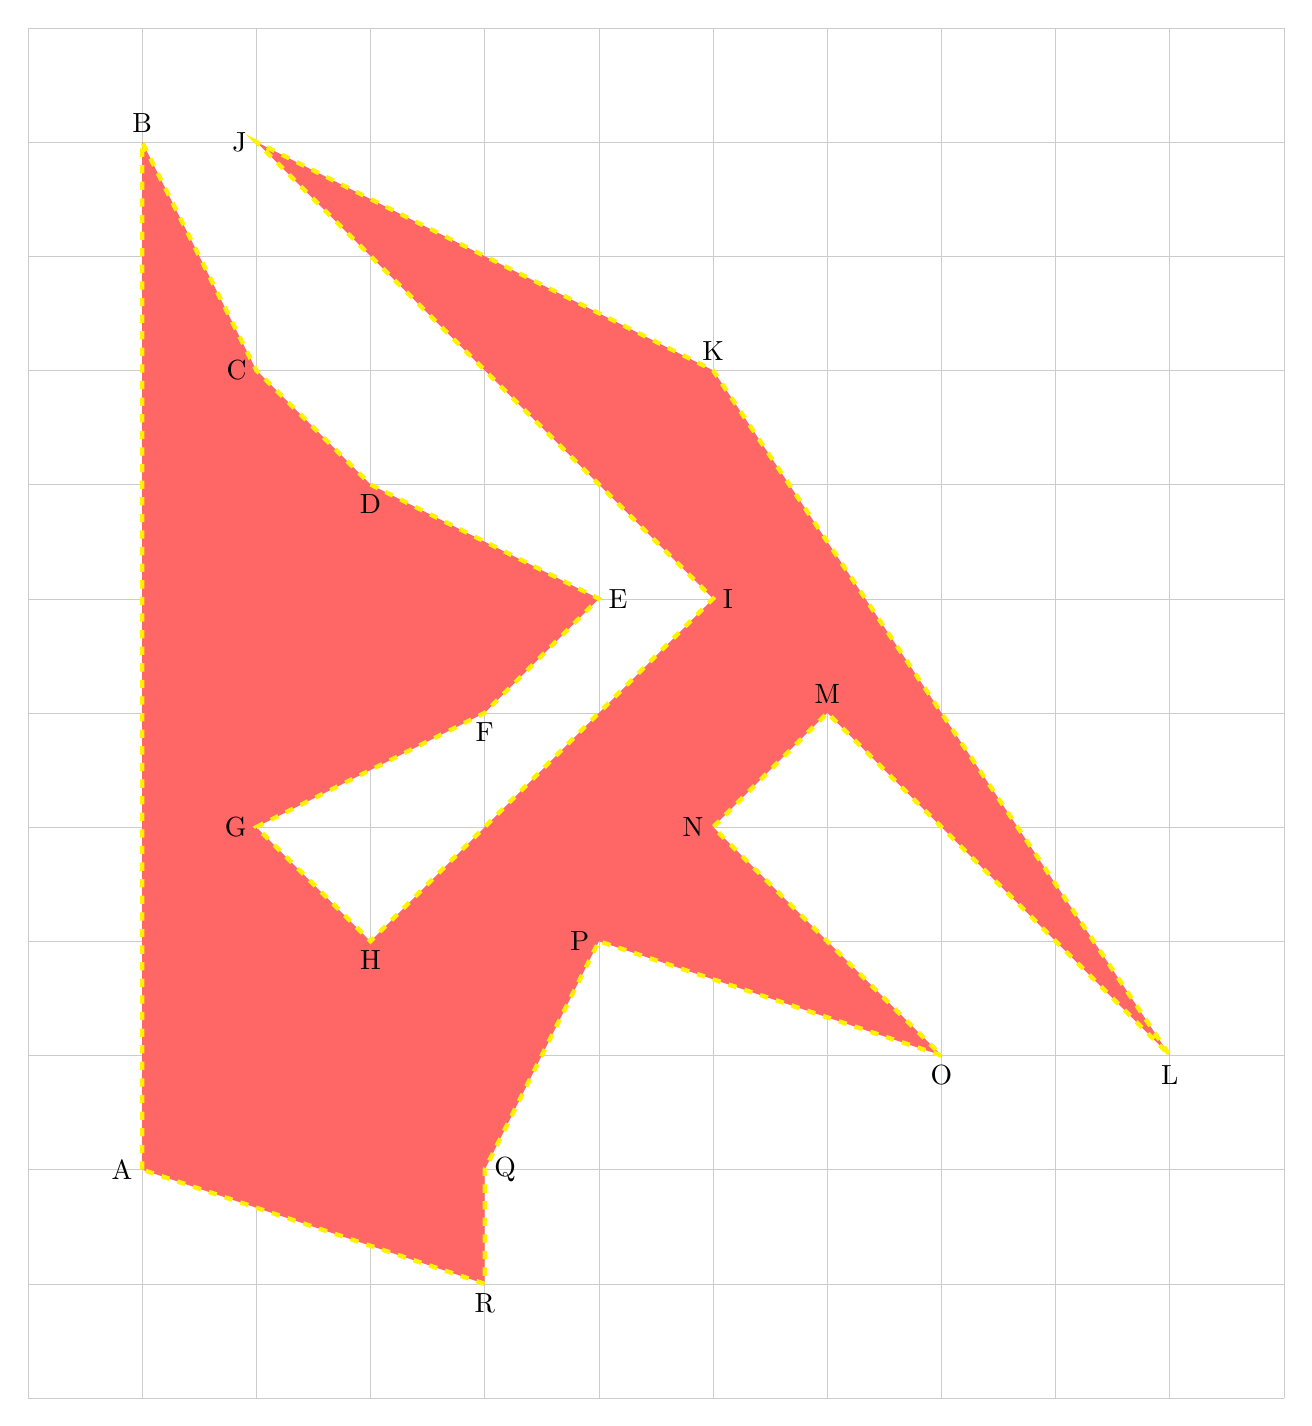
\begin{tikzpicture}[scale=1.45] 
\draw [help lines, black!20] (0,-1) grid (11,11);
\coordinate (A) at (1,1);
\coordinate (B) at (1,10);
\coordinate (C) at (2,8);
\coordinate (D) at (3,7);
\coordinate (E) at (5,6);
\coordinate (F) at (4,5);
\coordinate (G) at (2,4);
\coordinate (H) at (3,3);
\coordinate (I) at (6,6);
\coordinate (J) at (2,10);
\coordinate (K) at (6,8);
\coordinate (L) at (10,2);
\coordinate (M) at (7,5);
\coordinate (N) at (6,4);
\coordinate (O) at (8,2);
\coordinate (P) at (5,3);
\coordinate (Q) at (4,1);
\coordinate (R) at (4,0);


\draw [ultra thick, yellow, dashed,fill=red!60]
(A)--(B)--(C)--(D)--(E)--(F)--(G)--(H)--(I)--(J)--(K)--(L)--(M)--(N)--(O)--(P)--(Q)--(R)--(A);
\node [left] at (A) {A};
\node [above] at (B) {B};
\node [left] at (C) {C};
\node [below] at (D) {D};
\node [right] at (E) {E};
\node [below] at (F) {F};
\node [left] at (G) {G};
\node [below] at (H) {H};
\node [right] at (I) {I};
\node [left] at (J) {J};
\node [right,above] at (K) {K};
\node [below] at (L) {L};
\node [above] at (M) {M};
\node [left] at (N) {N};
\node [below] at (O) {O};
\node [left] at (P) {P};
\node [right] at (Q) {Q};
\node [below] at (R) {R};
\end{tikzpicture}
\end{center}

\newpage
\begin{tikzpicture}[scale=2,xscale=1.2]
\draw [help lines, black!10] (-1,-1) grid (6,11);

\path (0,0) coordinate(A) [below] node {A};
\path (0,10) coordinate(B) [above] node {B};
\path (2,10) coordinate(C) [above] node {C};
\path (0,6) coordinate(D) [left] node {D};
\path (2,6) coordinate(E) [above] node {E};
\path (2,0) coordinate(F) [below] node {F};
\path (1,9) coordinate(G) [left] node {G};
\path (1,7) coordinate(H) [below] node {H};
\path (1,5) coordinate(I) [above] node {I};
\path (1,1) coordinate(J) [left] node {J};
\path (2,5) coordinate(K) [above] node {K};
\path (2,1) coordinate(L) [below] node {L};
\path (2,9) coordinate(M) [above] node {M};
\path (2,7) coordinate(N) [below] node {N};

\draw (F)--(A)--(B)--(C);
\draw (D)--(E);
\draw (L)--(J)--(I)--(K);
\draw (N)--(H)--(G)--(M);

\draw (C) arc (90:-90:2);
\draw (M) arc (90:-90:1);

\draw (K) arc (90:-90:2);
\draw (E) arc (90:-90:3);
\end{tikzpicture}

\end{document}
